\documentclass[11pt]{article}
\usepackage[margin=0.8in]{geometry}
\usepackage{graphicx,booktabs,longtable,amsmath,array}
\usepackage[T1]{fontenc}
\usepackage[hidelinks]{hyperref}
\newcommand{\runpath}{../outputs/baseline_moon}
\graphicspath{{../outputs/baseline_moon/figures/}}
\title{Galactic supernova follow-up with Rubin\\\large A neutrino-triggered Monte Carlo forecast}
\author{GalSNRubin simulation}
\date{Baseline experiment: triggers in 2027}
\begin{document}
\maketitle
\begin{abstract}
We simulate 1,000 catalogue-sampled Galactic supernova locations and trigger dates
for each of three canonical progenitors (RSG, BSG and WR). The same candidates
are reused across the three models. GNILC-rescaled dust extinction feeds the
existing early light-curve package; an idealized Rubin search then includes
night, source altitude, a configurable Moon exclusion, setup, pointing
probability, exposure depth and
saturation. This is a conditional forecast of an idealized response, not an
operational scheduler or an estimate of the Galactic supernova rate.
\end{abstract}

\section{Baseline results}
\begin{center}\small\input{\runpath/results.tex}\end{center}
Counts of saturated-only detections and usable photometry are out of all 1,000
triggers per type. Median times and magnitudes are conditional on detection.
Saturated-only means every detected exposure was saturated: no usable detection
was obtained. Usable means at least one detected, unsaturated exposure was
obtained, even if longer or later exposures saturated. These two categories
partition the detections. Discovery magnitudes
are underlying model magnitudes, even where detector saturation prevents
ordinary PSF photometry. We optimistically count saturated sources as localized.

Correcting the former stop at the first saturated exposure and the event classification changes
the saturated-only counts from 702 to 521 (RSG), 708 to 485 (BSG), and 674 to 423
(WR). Much of this change retains events that already had usable photometry;
continuing past saturated long exposures additionally recovers usable data for
2 BSG and 22 WR events. Detection totals, first-detection times and discovery
magnitudes are unchanged for the same paired sample.

In this baseline, 148 candidates per type exceed the minimum altitude at
transit but have no nighttime window. The $10^\circ$ Moon cut reduces the
available pointing count for 15 of the 1,000 shared candidates, but leaves
some complete pointings for each: the exclusive Moon-avoidance category is
therefore zero. Relative to the saved run without lunar avoidance, two WR
detections are lost because the remaining exposures fall outside the valid
emission interval; these count as no valid model exposure. RSG and BSG
detection totals are unchanged, although discovery times and saturation
statistics can change.

\begin{figure}[!htbp]\centering
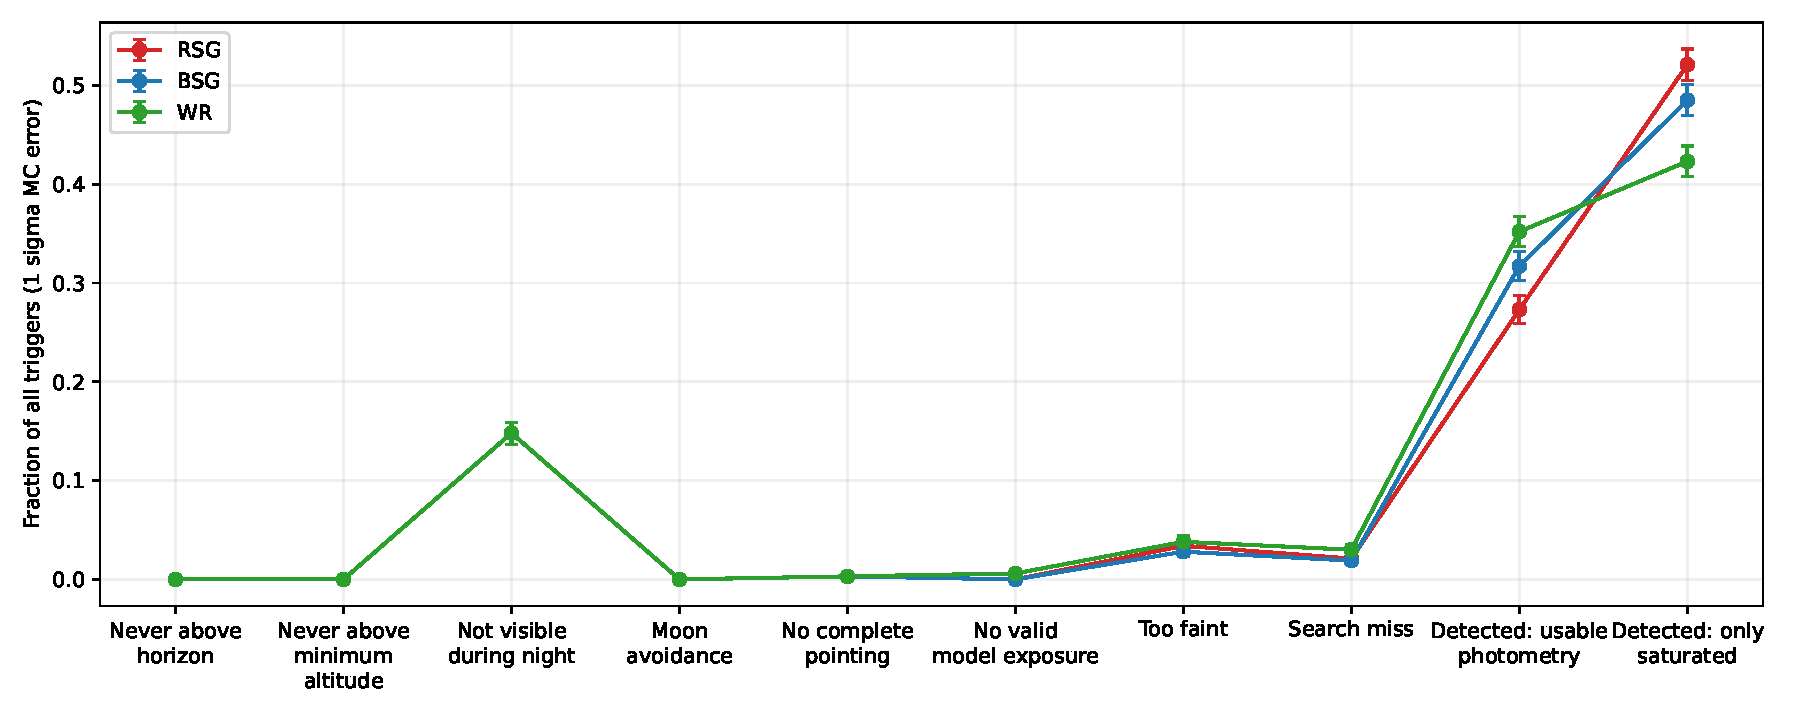
\includegraphics[width=\linewidth]{outcomes.pdf}
\caption{Exhaustive, mutually exclusive terminal outcomes. Error bars are
binomial Monte Carlo standard errors; the three classes share input draws and
are correlated. ``Not visible during night'' means the source exceeds the
minimum altitude at transit but has no night/altitude window before the
deadline. ``Moon avoidance'' means such windows could accommodate a complete
pointing without the Moon cut, but none can with it. Physical and operational
systematics are not in these errors.}
\end{figure}

\section{Population and emission model}
The input is \texttt{TRILEGAL\_noLMCSMC\_10plusZAMS.pkl}, a trusted local pandas
pickle with 39,723 rows. Rows are sampled uniformly with replacement, preserving
their ICRS coordinates and distance moduli. Distances follow
$d/{\rm kpc}=10^{(\mu_0-10)/5}$. The catalogue's extinction and stellar masses are
not used for the model: \texttt{galdust.av(ra,dec,d)} supplies $A_V$ to
\texttt{ccsnlc.LightCurveModel}. Thus the population is a spatial weighting,
not an evolutionary selection of each progenitor class.

The existing light-curve library supplies its canonical RSG, BSG and WR
progenitors, neutrino-to-breakout delays, shock-cooling emission, light-travel
smearing, blackbody spectrum, CCM extinction and LSST throughput integration.
Its assumptions and literature provenance are documented in the sibling
\texttt{CCLightCurves/README.md}; the dust model is documented in
\texttt{DustModel/galdust-repo/README.md}. The baseline uses deterministic delays.
No extrapolation is made beyond the library's $T=1$ eV cutoff. Pre-breakout
flux is zero; post-cutoff emission is unknown, not zero. In particular, a WR
non-detection after model expiry is not evidence against later optical emission.

\section{Visibility and observing policy}
Trigger dates are uniform in UTC over 2027. Rubin coordinates and field area
come from the official observatory pages\footnote{\url{https://rubinobservatory.org/for-scientists/rubin-101}}
\footnote{\url{https://rubinobservatory.org/for-scientists/rubin-101/instruments}}.
We first reject sources with maximum geometric altitude at or below the horizon,
then sources that never exceed the minimum altitude. A night starts ten minutes
after evening astronomical twilight and ends at morning astronomical twilight.
A source must be above the minimum altitude during that night. A three-day
follow-up deadline is measured from the trigger, not from the first exposure.
The date range can cross into 2028 for late-December triggers. Sources that
exceed the altitude threshold at transit but have no such nighttime window
are classified as ``not visible during night,'' separately from sources that
never reach the altitude threshold.

Within those windows, the angular separation between the source and the
topocentric Moon must be at least $10^\circ$ in the baseline. The exclusion
radius is configurable through \texttt{moon\_avoidance\_deg}; zero disables
the cut. The veto is independent of lunar phase and applies to the full
pointing block. It is a geometric exclusion only: lunar sky brightening
outside the avoidance region is not modelled.

Astropy supplies Sun and Moon positions, Earth rotation and CIRS coordinates.
The Moon uses Astropy's offline builtin ephemeris and the observatory's
topocentric CIRS frame, including lunar parallax. A source's
CIRS coordinates are frozen at trigger time for its short follow-up; a 300 s
solar/lunar/rotation grid is interpolated (with unwrapped lunar right ascension).
Visibility boundaries are rounded inward on a 60 s grid; sub-step windows or
lunar crossings may be unresolved. Refraction is disabled.
Future Earth orientation uses bundled IERS data with no downloads; polar motion
beyond the prediction range defaults to a long-term mean, with arcsecond-scale
accuracy. This is adequate for the present timing resolution.

The initial 90 s filter setup starts at the first eligible instant. It is charged
once; it may complete during a subsequent gap. Each pointing contains
$1,1,15,15$ s exposures, each followed by 15 s dead time including repositioning:
$T_{\rm point}=92$ s. Only complete blocks fitting within a visibility window are
scheduled, including the last dead time. Observing pauses across daylight or
low-altitude or Moon-excluded intervals and resumes in the next eligible window.

\section{Localization and photometry}
We interpret the prescribed uncertainty as a spherical-cap \emph{radius}:
\begin{align}
\theta(d)&=\min\left[180^\circ,30^\circ(d/25\,{\rm kpc})^2\right],\\
A(\theta)&=2\pi(1-\cos\theta)(180/\pi)^2\;{\rm deg}^2,\\
p_{\rm hit}&=\min(1,9.6\,{\rm deg}^2/A).
\end{align}
Each pointing draws independently with replacement. Its exposures share one
FOV result; this is not a tiling without replacement. Source visibility is
assessed at the true source coordinates, including the Moon veto. No trigger
centroid or probability-map visibility is generated. Consequently this is an idealized area-ratio search,
not a deployable localization strategy. The search uniforms are paired between
progenitor types for each candidate. After the first detection the telescope
tracks the known source. Consecutive exposures are evaluated individually in
time order, with no independent search draw within a pointing. A saturated
long exposure does not stop observations while short exposures can still be
usable. We finish the first pointing in which \emph{all} exposures saturate,
then stop; otherwise we continue to the deadline. Model-expired exposures
cannot produce detections or establish saturation.

Event classification retains the full observed history. Any detected,
unsaturated exposure makes the outcome \texttt{detected\_unsaturated}, including
when a subsequent pointing saturates in every exposure. Only a source with
detections but no usable exposure is \texttt{detected\_saturated}. Thus a source
that jumps from undetectable to saturated in both short and long exposures
without an observed usable interval is saturated-only. If the first short
exposures are too faint and the following long exposures saturate, the next
pointing is still attempted: its short exposures may supply usable photometry.
The baseline long integration consists of two separate 15 s exposures, not a
coadded 30 s measurement; the same rule applies to configured 1 s and 30 s
exposures. Saturation in 30 s alone would not disqualify a usable 1 s detection.

Five midpoint samples integrate flux over each exposure. Any exposure crossing
the model cutoff is invalid. Single-exposure detection requires SNR $\geq5$;
no coaddition or repeat confirmation is required. The discovery time is the
exposure end, with no image-processing latency. Sensitivity follows Rubin's
SMTN-002 prescription\footnote{\url{https://smtn-002.lsst.io/}}:
\begin{equation}
{\rm SNR}=\frac{C}{\sqrt{C+n_{\rm eff}(B+R^2+Dt)}},\qquad
n_{\rm eff}=2.266({\rm FWHM}_{\rm eff}/s_{\rm pix})^2.
\end{equation}
Here $C$ is source electrons, $B$ sky electrons per pixel, $R$ read noise, $D$
dark current and $t$ exposure duration. Tabulated zero points convert AB flux to
counts. Dark sky and zenith seeing are fixed. Historical Science Book saturation
fiducials\footnote{\url{https://www.lsst.org/sites/default/files/docs/sciencebook/SB_Whole.pdf}}
are treated as configurable 15 s thresholds, scaled at constant charge by
$m_{\rm sat}(t)=m_{\rm sat}(15)+2.5\log_{10}(t/15)$.
These are planning assumptions rather than measured 2027 short-exposure performance.

\begin{figure}[!htbp]\centering
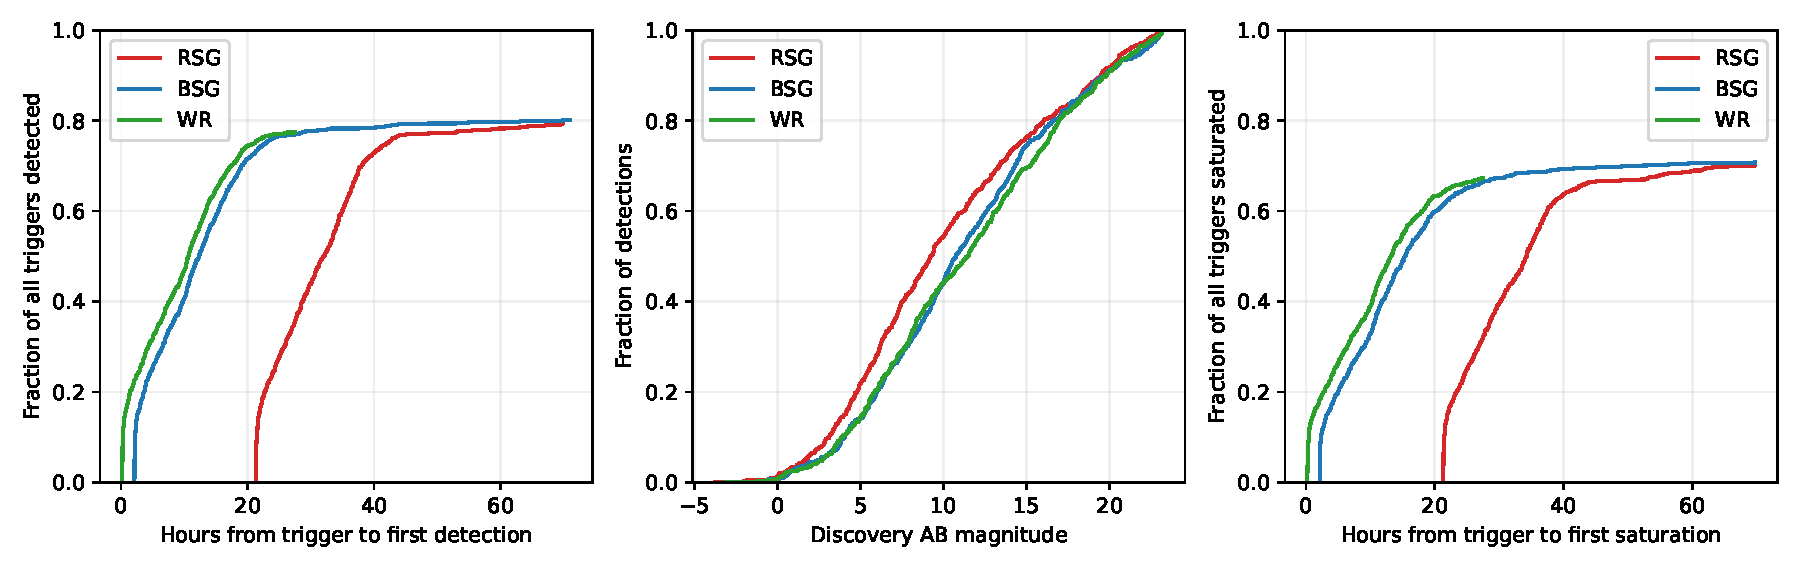
\includegraphics[width=\linewidth]{discovery.pdf}
\caption{Detection time, model brightness at discovery, and completion time of
the first fully saturated pointing. The latter is a stopping diagnostic and
can include sources with earlier usable photometry. Time distributions use all triggers as denominator and therefore retain
the incompleteness; brightness is conditional on detection. Three curves
compare progenitors using the same candidate population.}
\end{figure}
\begin{figure}[!htbp]\centering
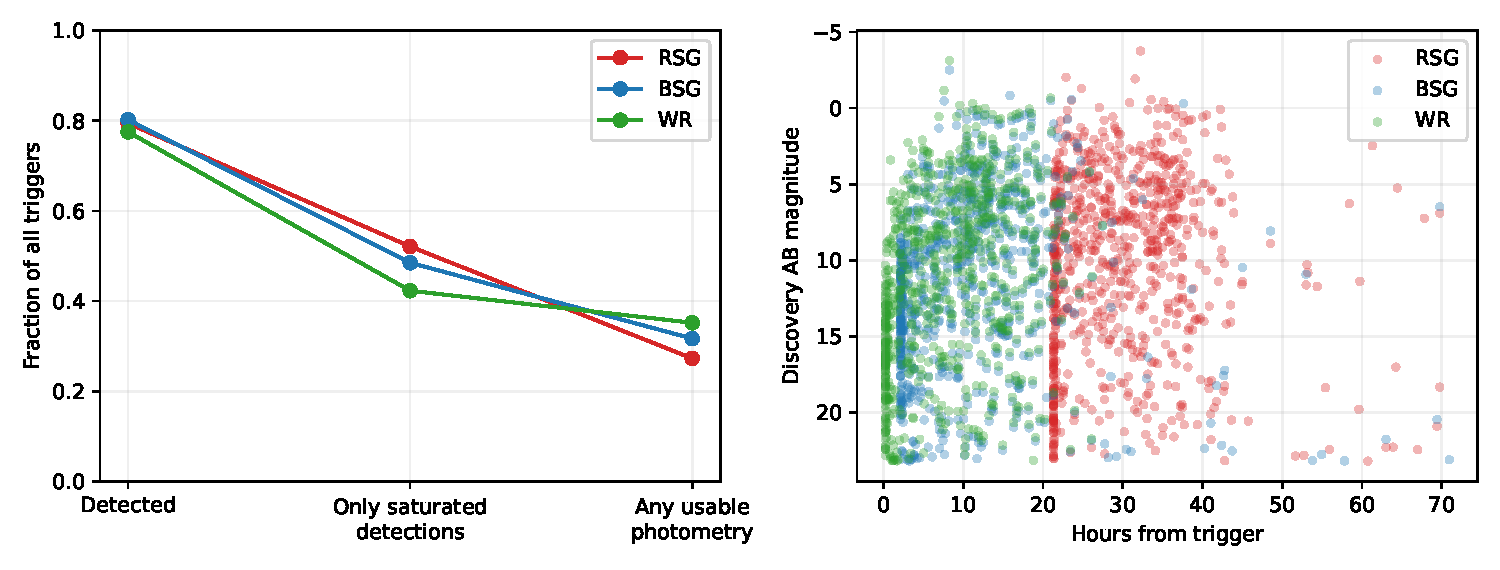
\includegraphics[width=\linewidth]{saturation.pdf}
\caption{Detection, saturated-only, and usable-photometry fractions, and the
relation between discovery time and brightness. The last two fractions sum to
the detected fraction. Saturated localization need not yield usable photometry.}
\end{figure}

\section{Miss accounting and limitations}
The ordered rejection reasons are: never above horizon; never above minimum
altitude; not visible during night within the deadline (before the lunar cut);
Moon avoidance; no complete pointing fits; no valid model exposure; too faint
in all valid exposures; and search miss despite at least one detectable
opportunity. Moon avoidance is assigned when complete pointings, including
setup and dead time, could fit without the lunar veto but none fit with it.
If the windows cannot fit a complete pointing even without the veto, the
outcome is instead no complete pointing. Partial lunar losses can delay or
reduce observations; events with remaining pointings retain their final
photometric or search outcome. These mutually exclusive reasons diagnose
the executed experiment, not a unique causal explanation in the real sky.
Model expiry is also retained as a separate event diagnostic for modelled events.
A detected source with any usable photometry remains an unsaturated success,
even if it later saturates. A saturated-only source is still counted as localized.

Weather, lunar sky brightening, other changing sky, airmass losses, crowding,
blending, template availability, pipeline failure, slew geometry, normal survey scheduling and
resource contention are omitted. At the 15-degree altitude threshold, using
zenith sensitivity is particularly optimistic. A 1 s exposure mode and recovery
of extremely saturated sources are assumed. Neither the smooth dust model nor
canonical progenitor spectra capture the full astrophysical uncertainty.
The curves quantify the stated model, not guaranteed Rubin performance.

\section{Sky distributions and extinction}
\begin{figure}[!htbp]\centering
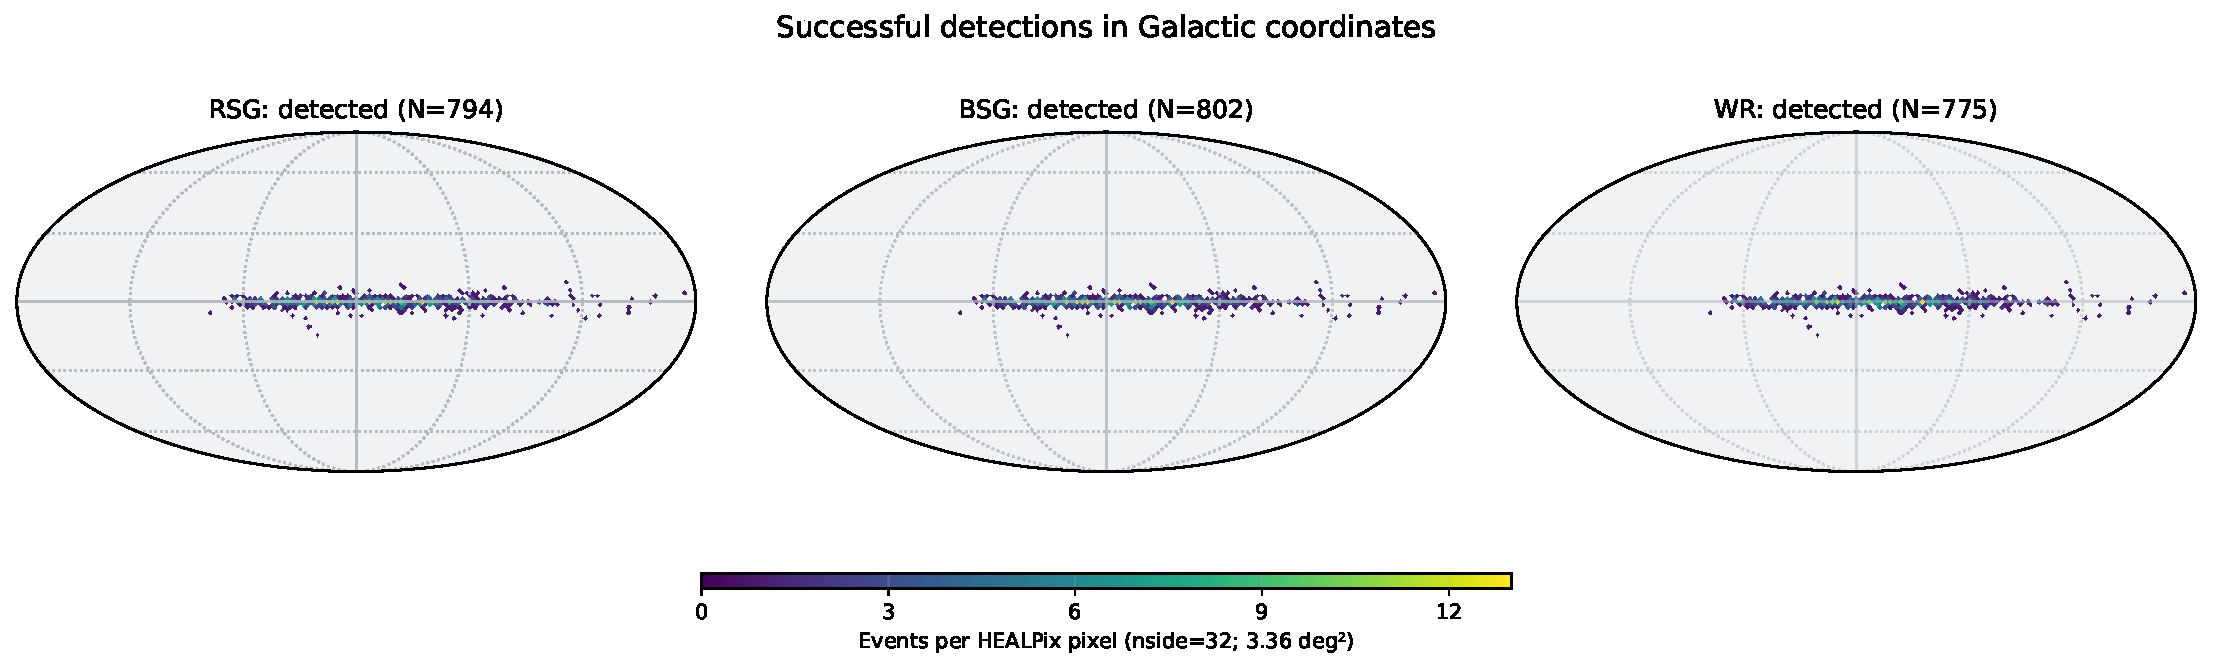
\includegraphics[width=\linewidth]{sky_success.pdf}
\caption{Successful supernova detections for each progenitor in Galactic
Mollweide projection. Saturated and unsaturated detections are both included.
The Galactic centre is at the centre; longitude increases to the left.
Graticules are spaced by $60^\circ$ in longitude and $30^\circ$ in latitude.
Colours count events in equal-area HEALPix pixels ($N_{\rm side}=32$,
3.36 square degrees per pixel), using a common scale across panels.
Light grey pixels contain no selected events. These are population counts,
not detection efficiencies.}
\end{figure}
\begin{figure}[!htbp]\centering
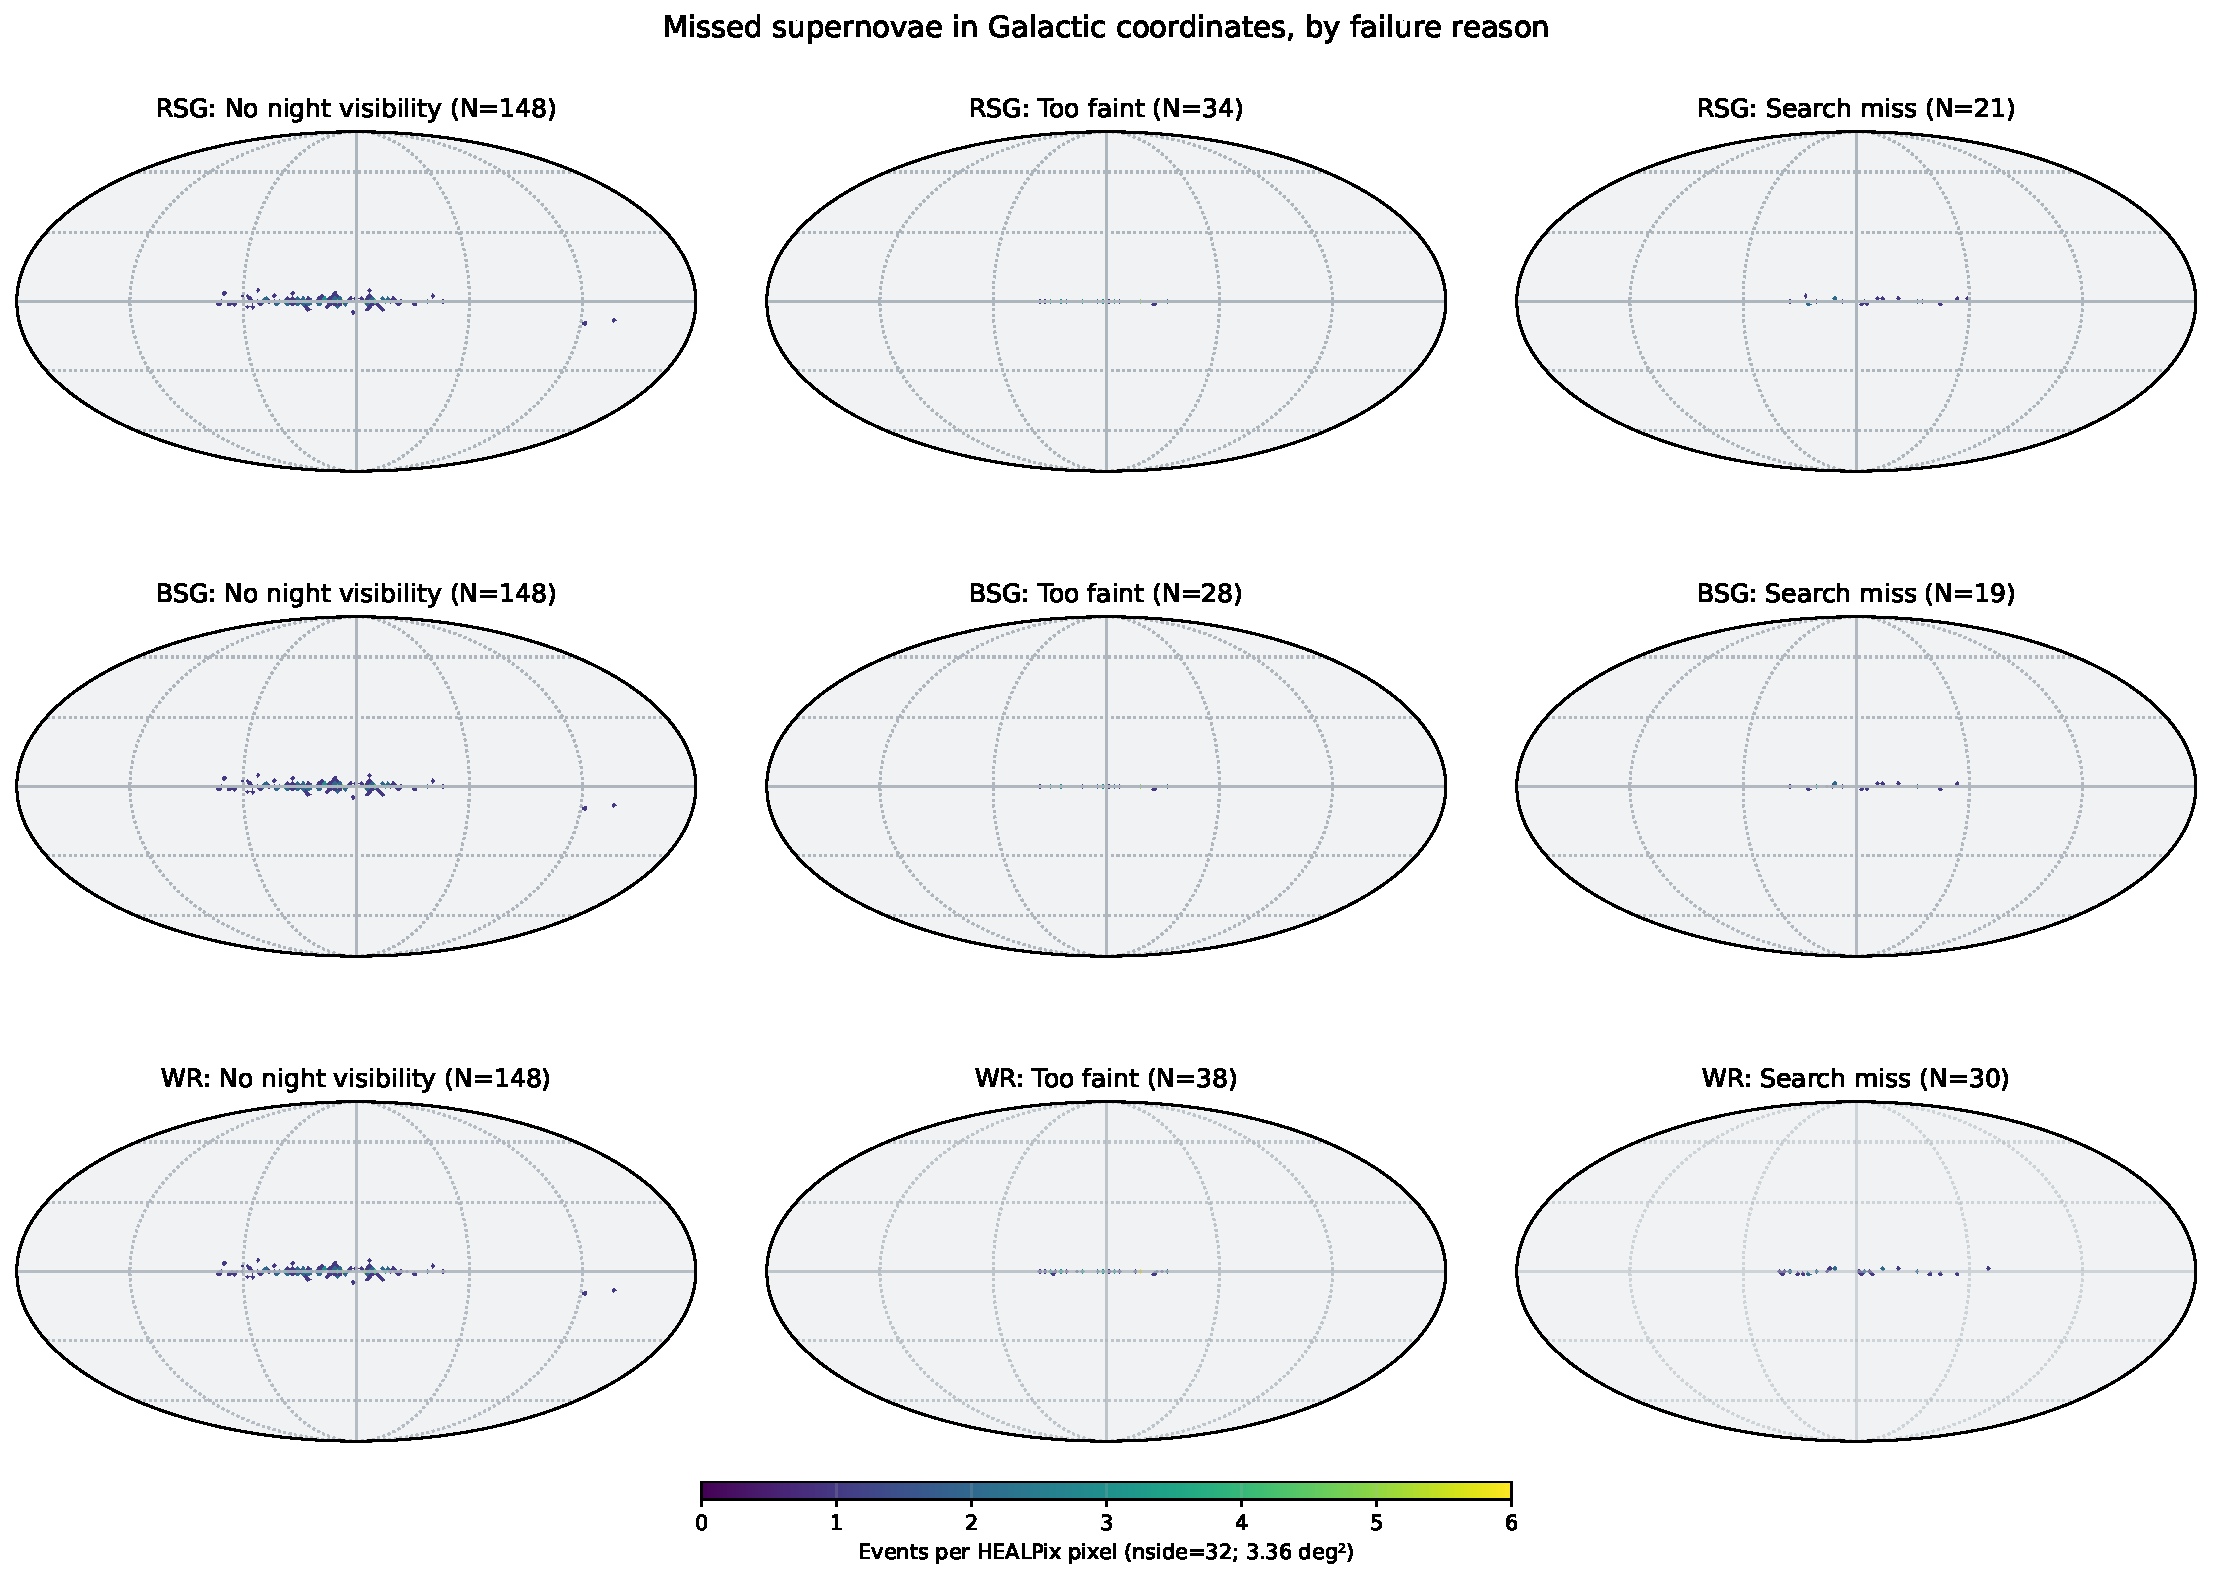
\includegraphics[width=\linewidth]{sky_failures.pdf}
\caption{Failure distributions in the same Galactic projection. Rows compare
progenitors; columns separate no night visibility, too faint, and search miss.
All nine panels use a common count scale, separate from the success figure.
Only the three requested failure categories are shown; other outcomes remain
in the complete accounting in Figure 1. The identical night-visibility panels
reflect the shared sky positions and trigger dates.}
\end{figure}
\begin{figure}[!htbp]\centering
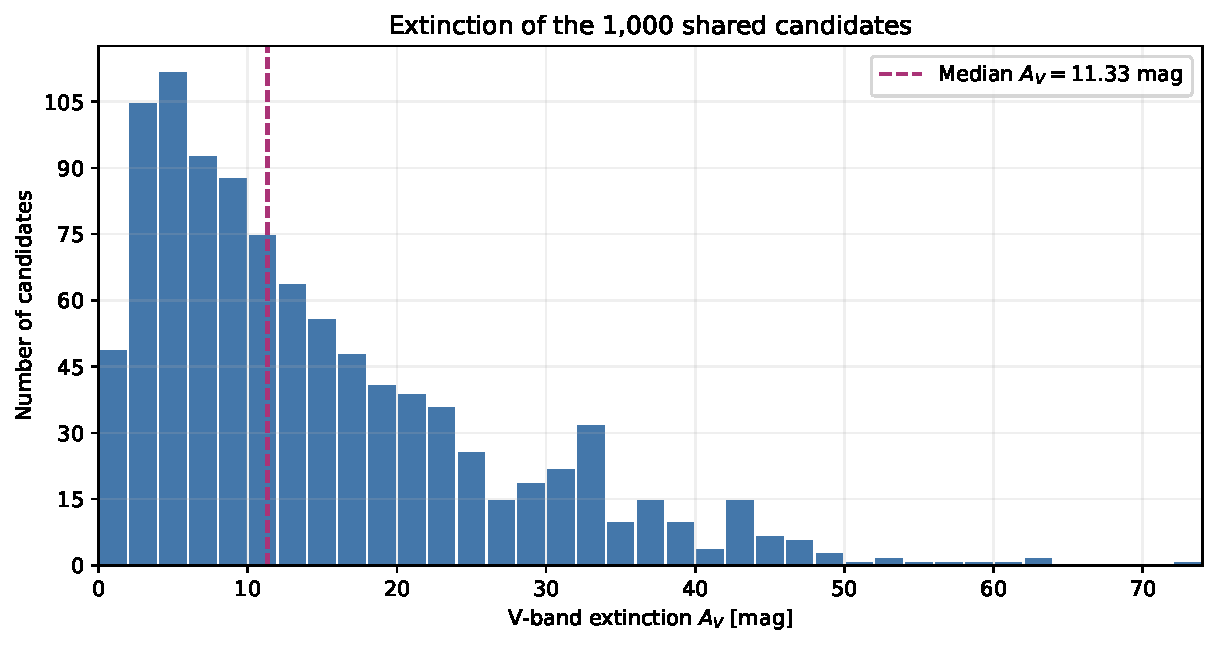
\includegraphics[width=.85\linewidth]{av_distribution.pdf}
\caption{Distribution of the dust model's V-band extinction $A_V$ for the
1,000 shared candidates, in 2 mag bins. Each candidate is counted once,
not once per progenitor; repeated catalogue draws are distinct candidates.
The dashed line marks the median. The full extinction range is included.}
\end{figure}
\clearpage
\section{Outcome dependence on candidate properties}
The following plots resolve every Figure 1 category as a function of distance,
Galactic latitude and longitude, dust extinction, UTC trigger month, localization
cap radius, and maximum geometric altitude. Within each bin, coloured fractions
use all triggers of that progenitor as the denominator, including successes;
thus occupied bins sum to unity. These are not fractions conditional on failure.
The bottom panel counts the shared candidates once each. Empty bins remain blank;
small counts imply large sampling uncertainty, and no error bands are shown.
All categories retain the same colours, including categories with zero counts.

These are descriptive marginal distributions of the catalogue-weighted sample.
Distance, extinction, sky position and localization area are correlated; the
plots do not isolate their separate causal effects. The localization radius is
itself a deterministic function of distance. Maximum altitude diagnoses geometric
accessibility, while trigger month probes seasonal night visibility. Galactic
longitude is wrapped to $[-180^\circ,180^\circ)$, with the Galactic centre at zero.
Bin edges, denominators, category counts and fractions are saved in
\texttt{figures/outcome\_trends.csv} within the run directory.

\begin{figure}[!htbp]\centering
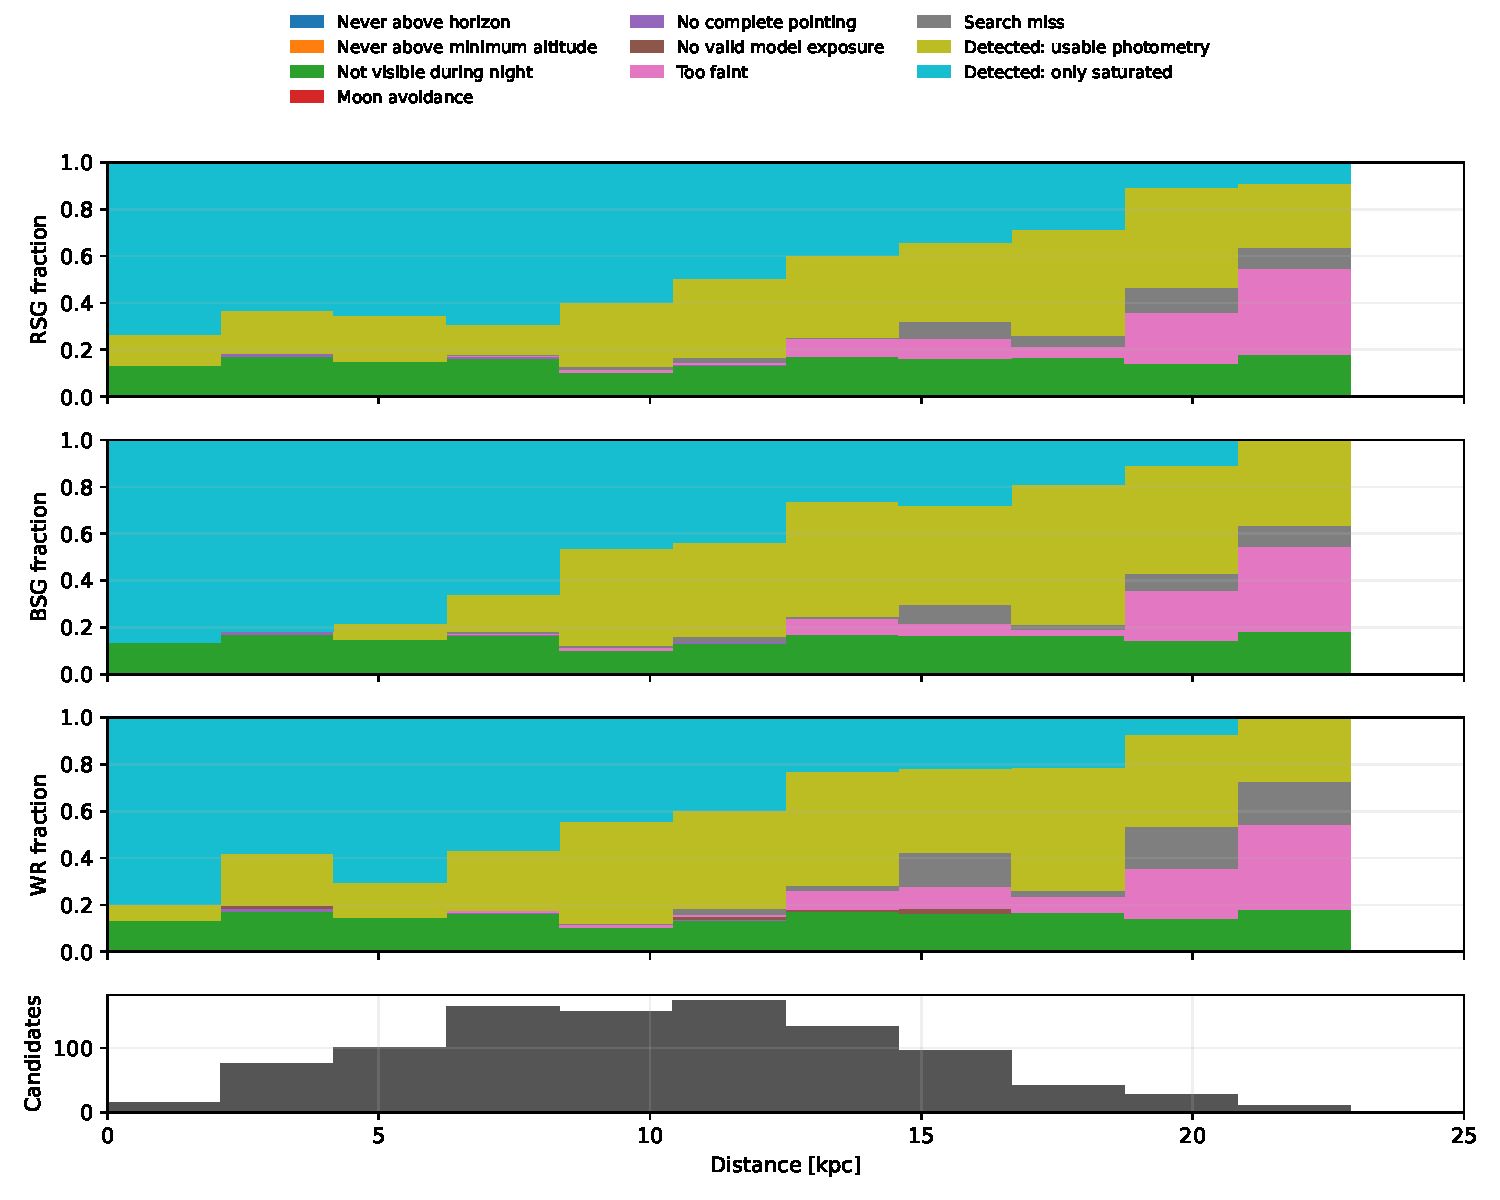
\includegraphics[width=\linewidth]{outcomes_by_distance.pdf}
\caption{Outcome fractions versus distance. Each progenitor panel includes all Figure 1 categories; the bottom panel gives the shared candidate count per bin. Blank bins have no candidates.}
\end{figure}

\begin{figure}[!htbp]\centering
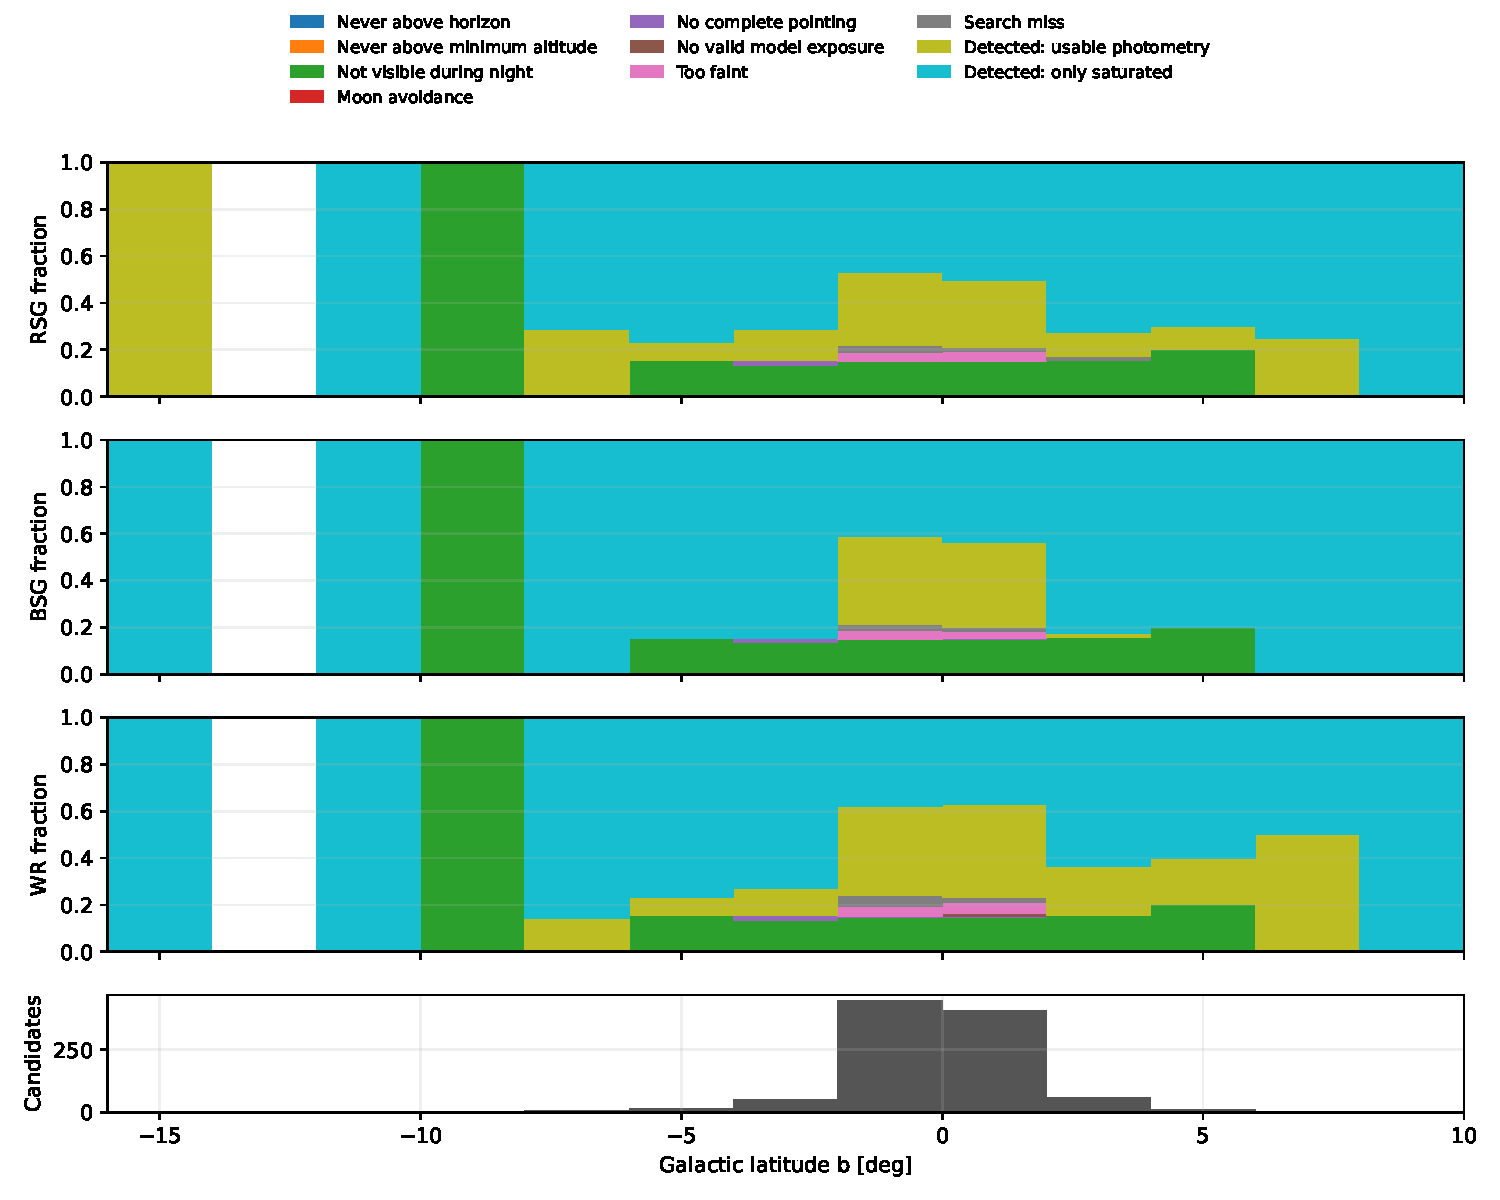
\includegraphics[width=\linewidth]{outcomes_by_latitude.pdf}
\caption{Outcome fractions versus Galactic latitude. Each progenitor panel includes all Figure 1 categories; the bottom panel gives the shared candidate count per bin. Blank bins have no candidates.}
\end{figure}

\begin{figure}[!htbp]\centering
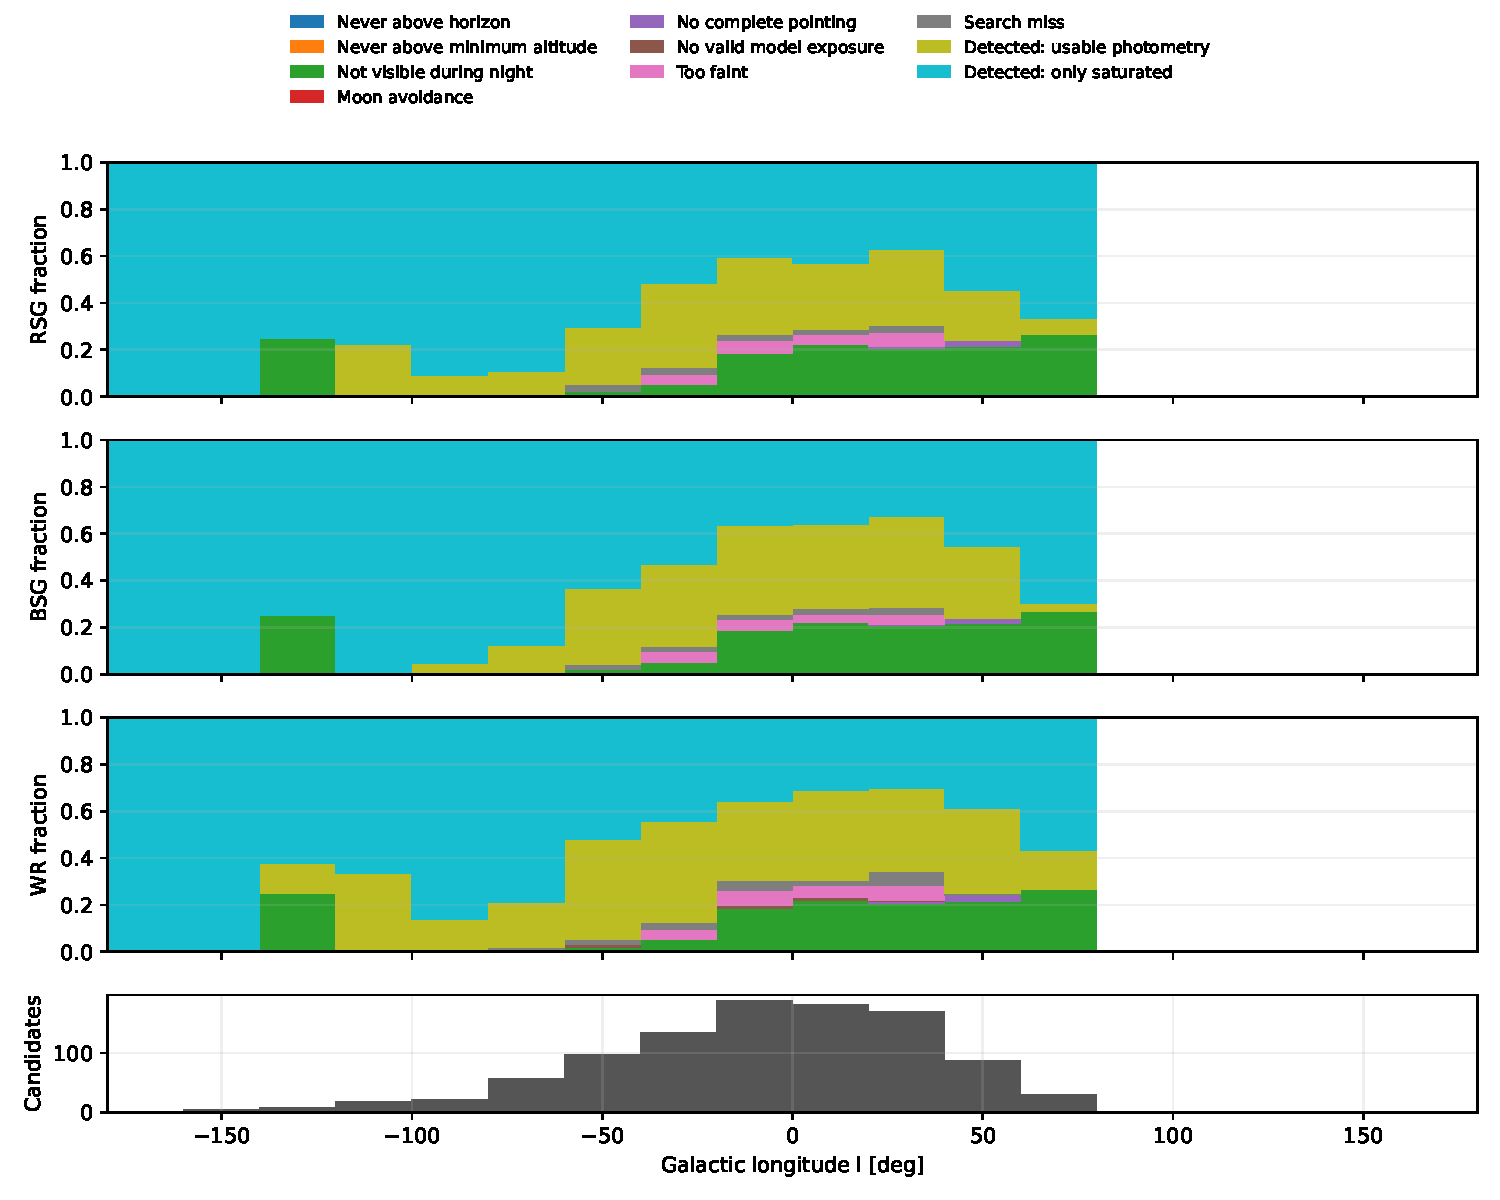
\includegraphics[width=\linewidth]{outcomes_by_longitude.pdf}
\caption{Outcome fractions versus Galactic longitude. Each progenitor panel includes all Figure 1 categories; the bottom panel gives the shared candidate count per bin. Blank bins have no candidates.}
\end{figure}

\begin{figure}[!htbp]\centering
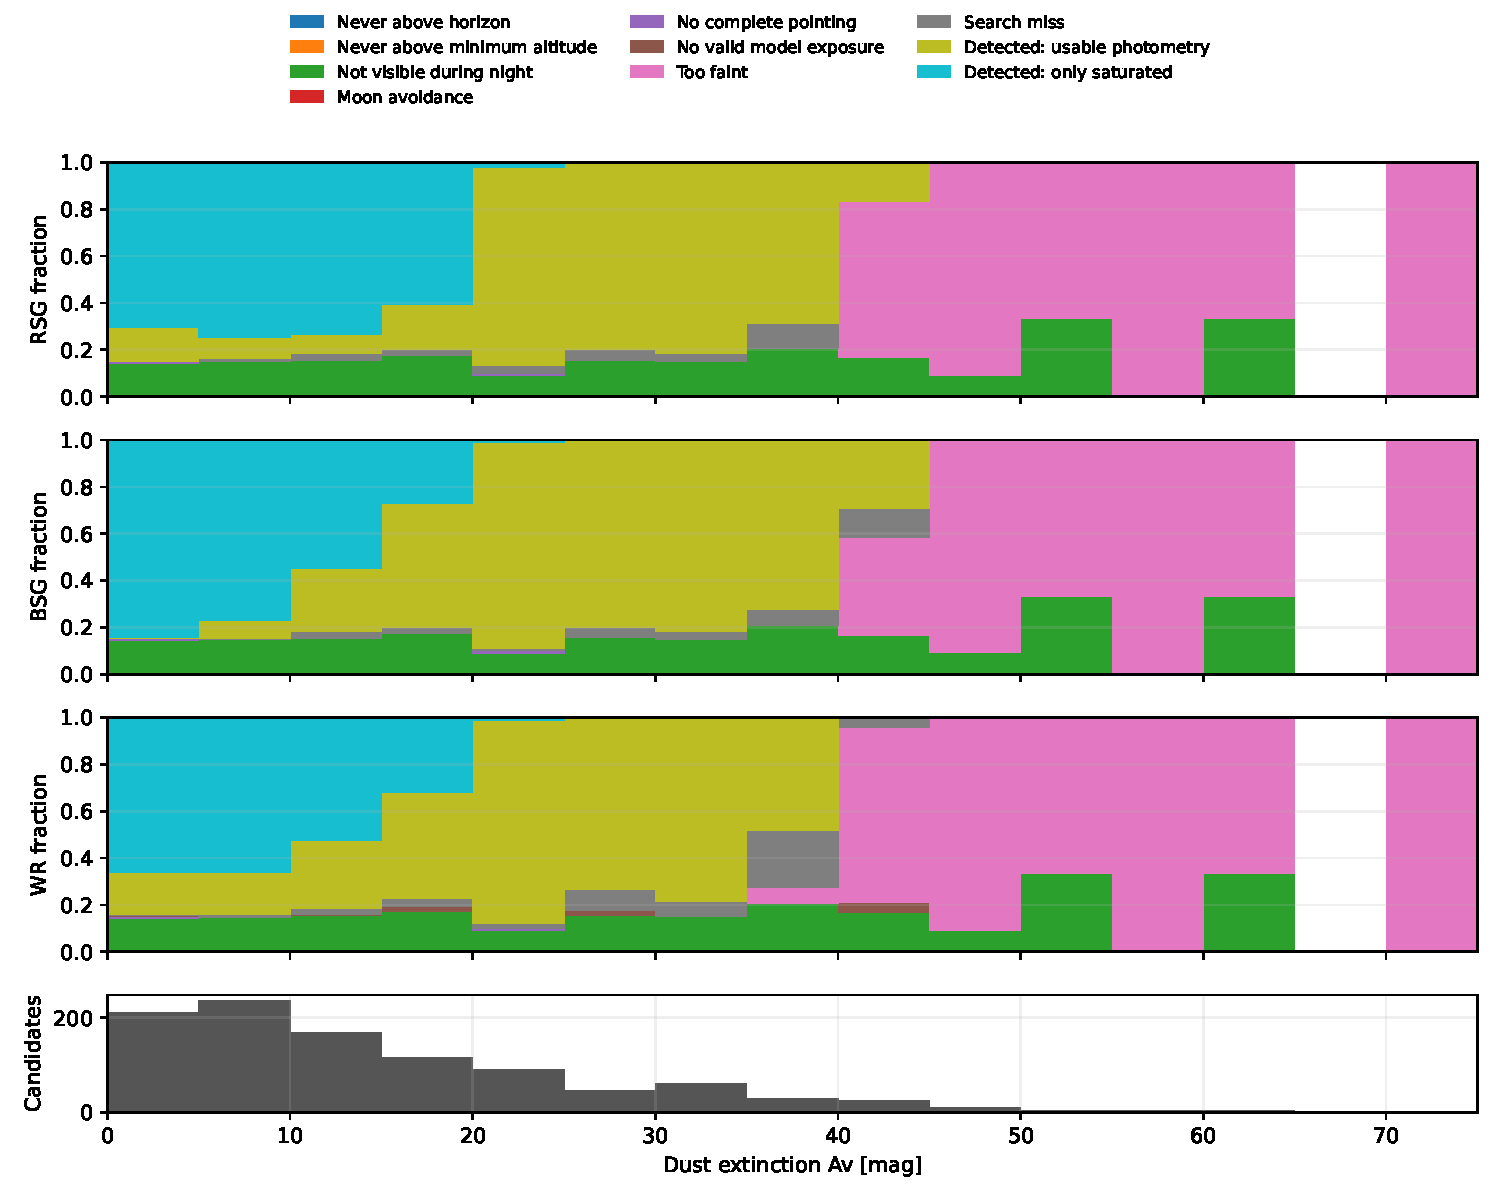
\includegraphics[width=\linewidth]{outcomes_by_extinction.pdf}
\caption{Outcome fractions versus dust extinction. Each progenitor panel includes all Figure 1 categories; the bottom panel gives the shared candidate count per bin. Blank bins have no candidates.}
\end{figure}

\begin{figure}[!htbp]\centering
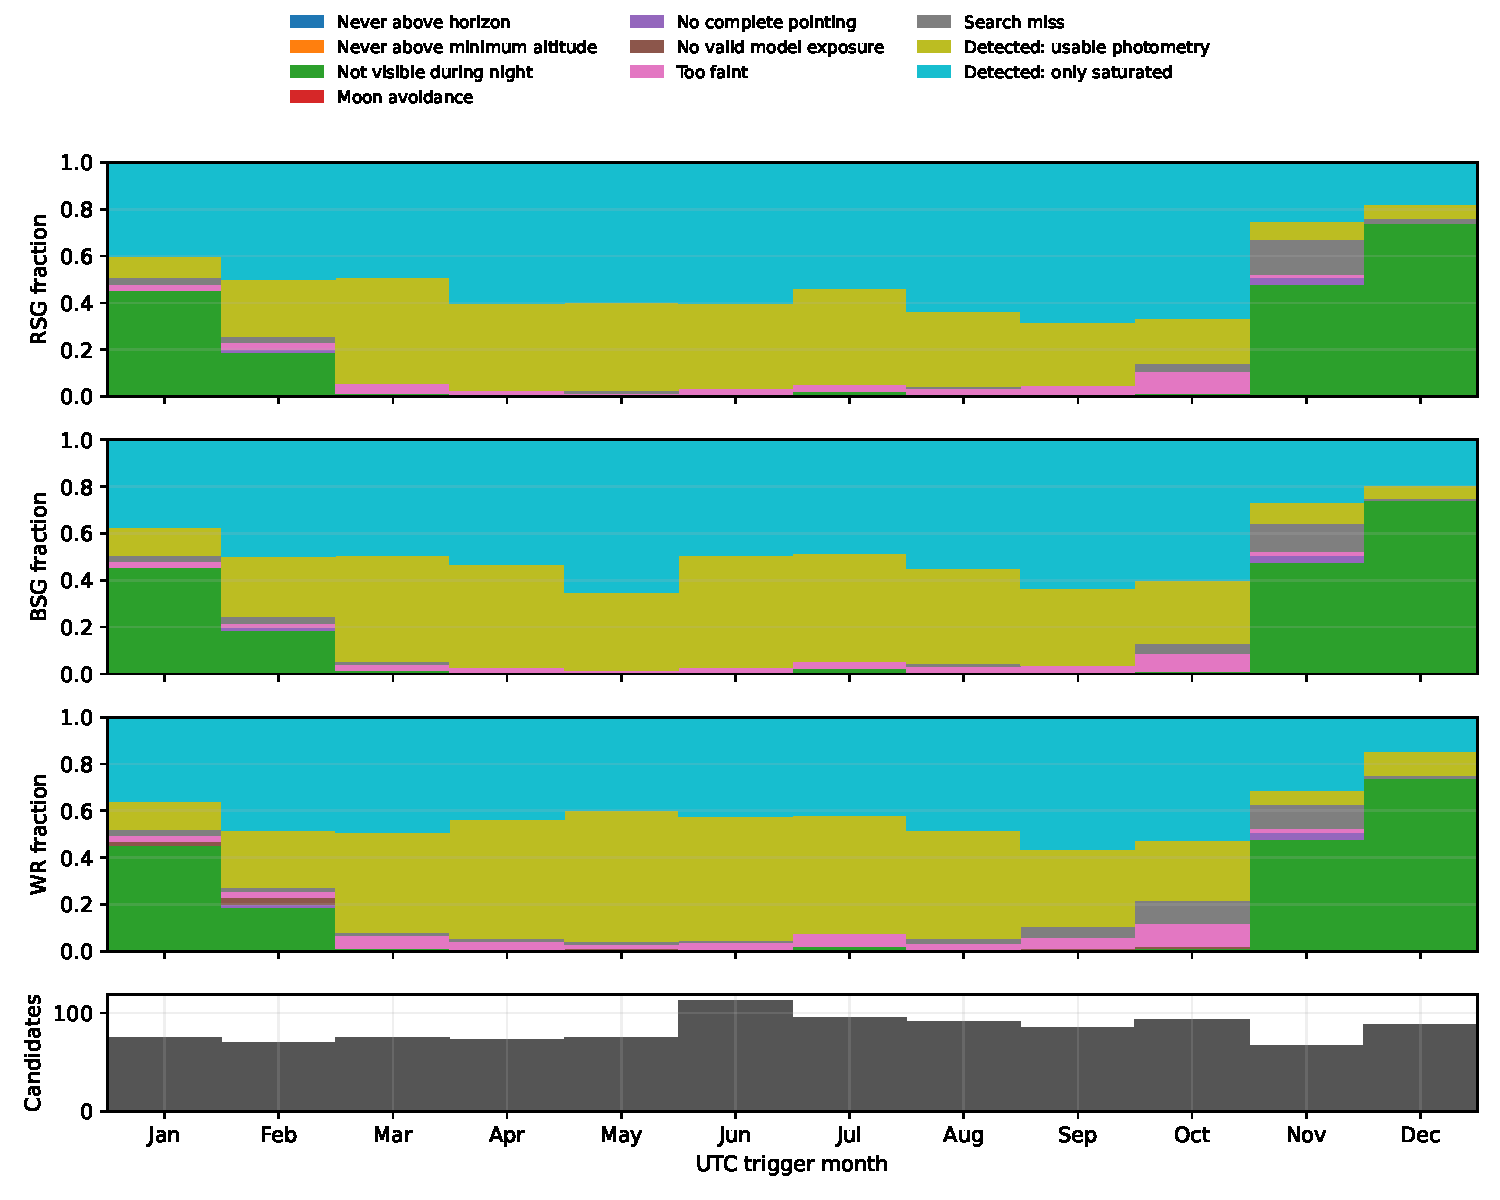
\includegraphics[width=\linewidth]{outcomes_by_month.pdf}
\caption{Outcome fractions versus UTC trigger month. Each progenitor panel includes all Figure 1 categories; the bottom panel gives the shared candidate count per bin. Blank bins have no candidates.}
\end{figure}

\begin{figure}[!htbp]\centering
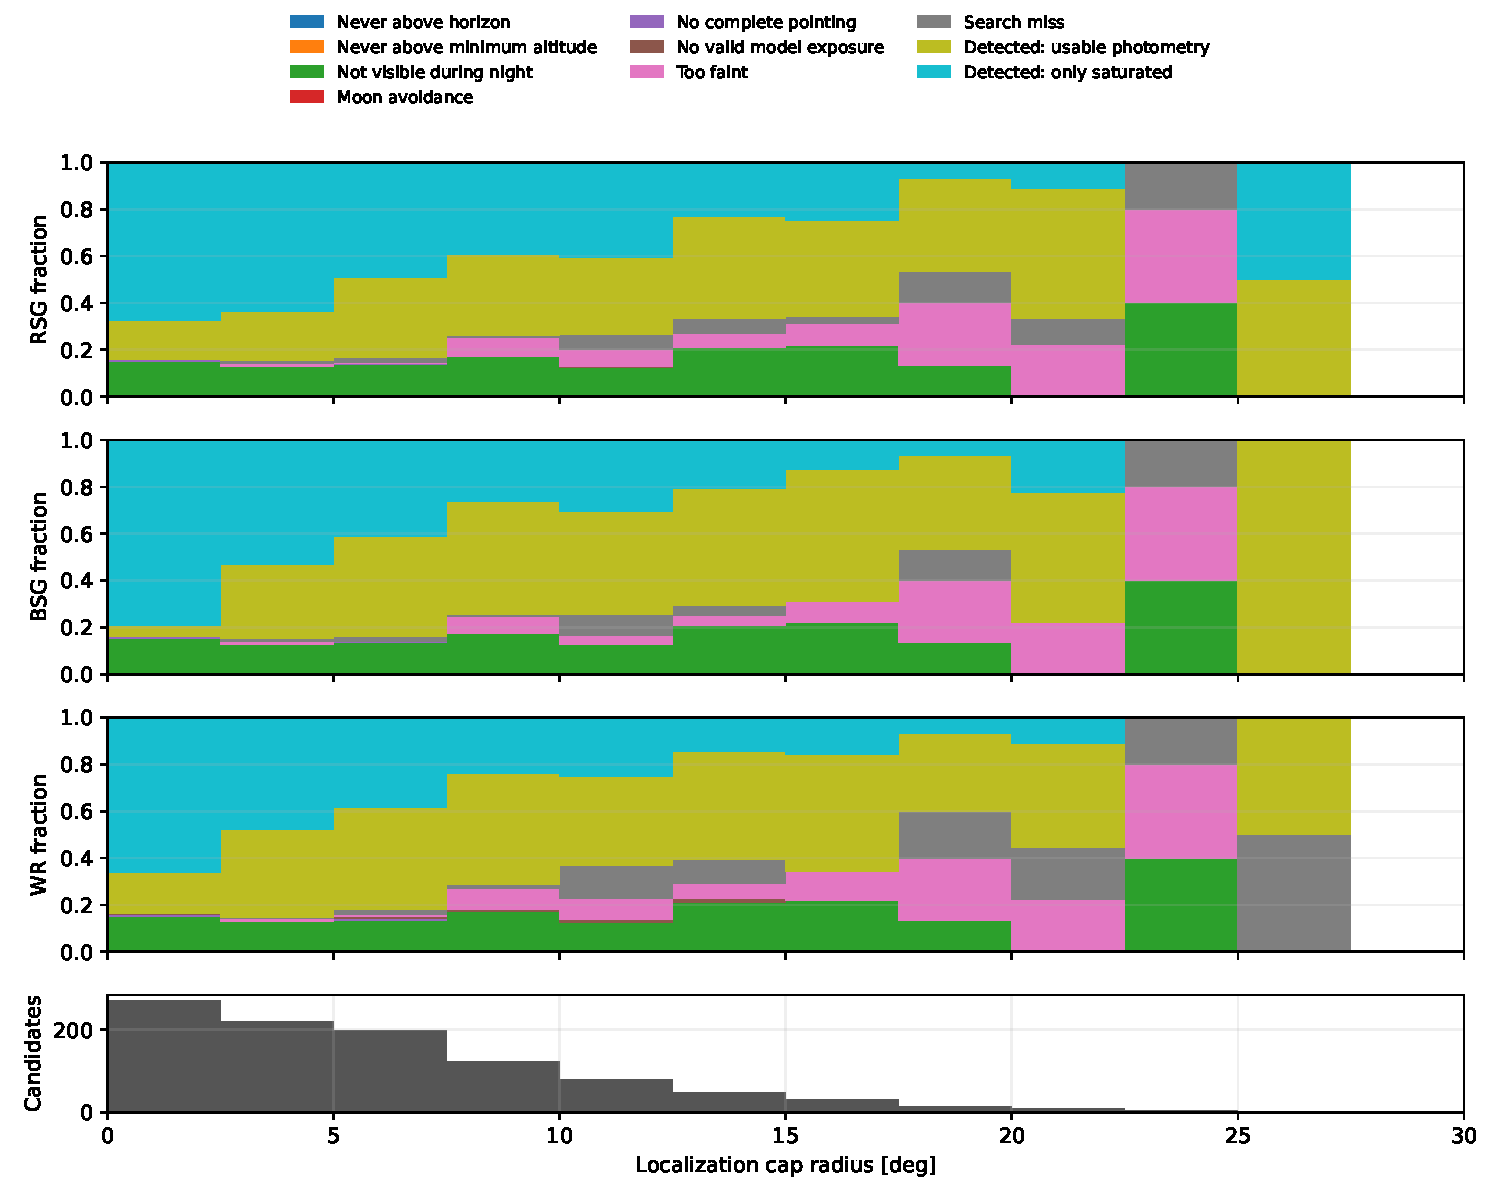
\includegraphics[width=\linewidth]{outcomes_by_localization.pdf}
\caption{Outcome fractions versus localization cap radius. Each progenitor panel includes all Figure 1 categories; the bottom panel gives the shared candidate count per bin. Blank bins have no candidates.}
\end{figure}

\begin{figure}[!htbp]\centering
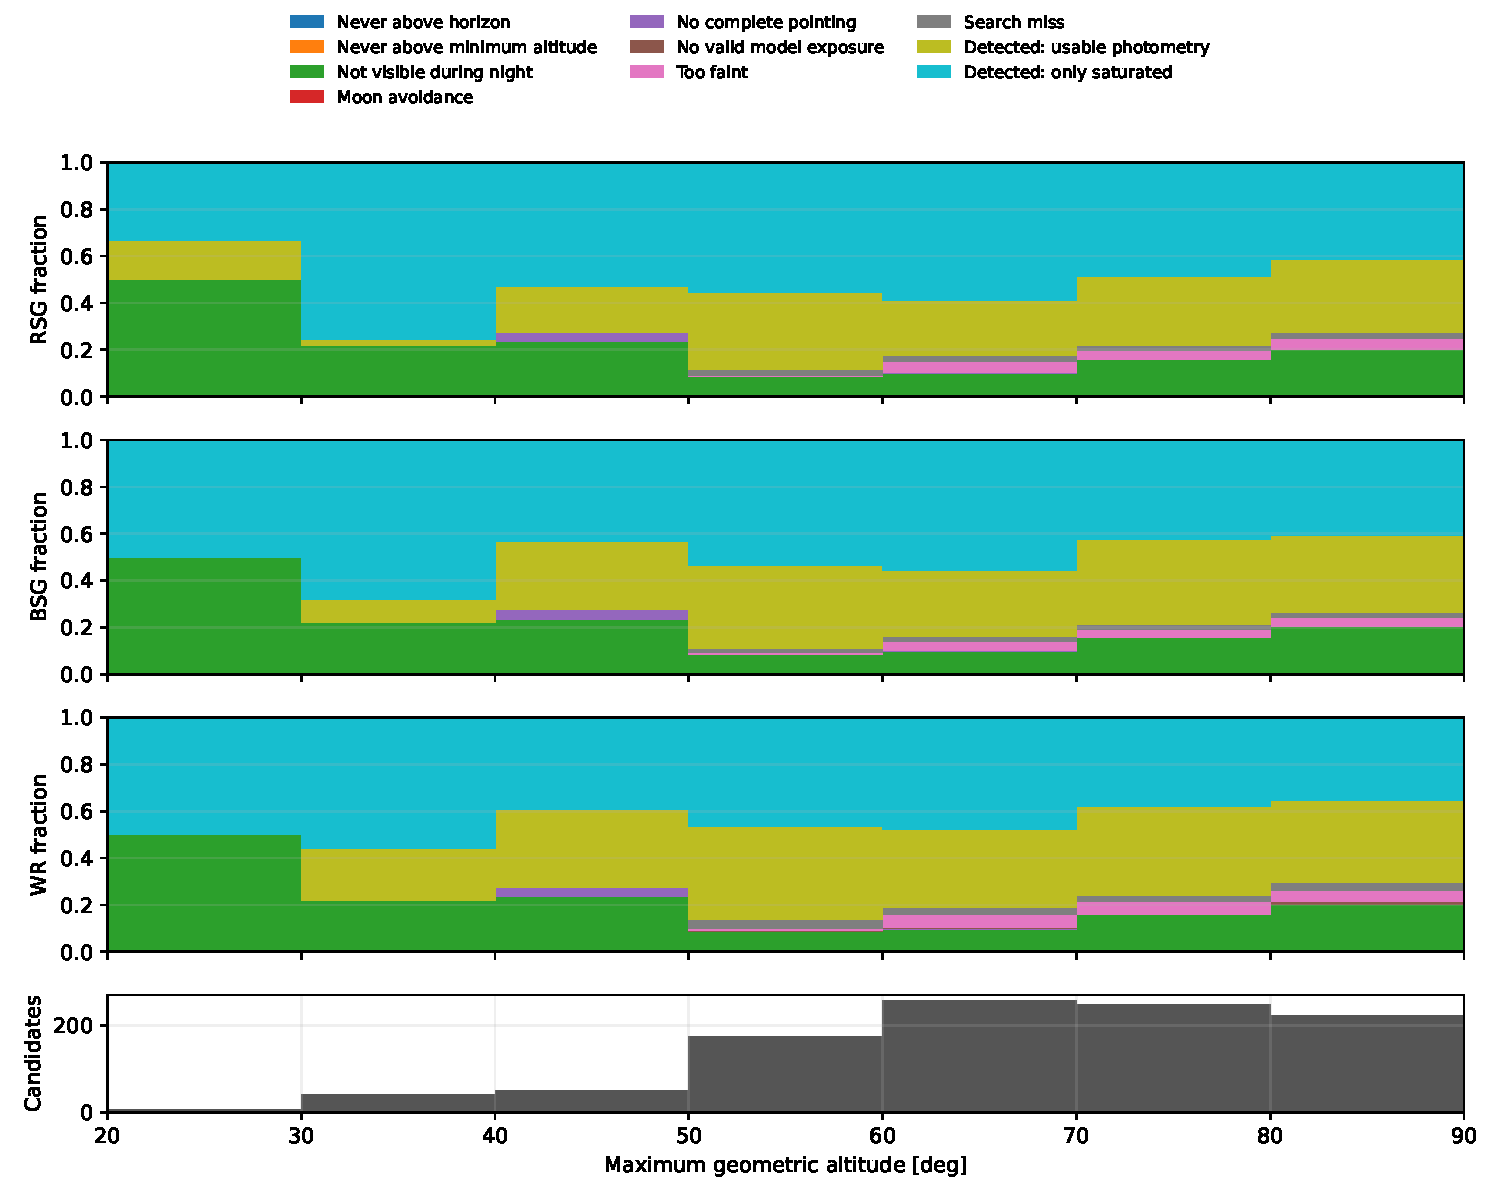
\includegraphics[width=\linewidth]{outcomes_by_altitude.pdf}
\caption{Outcome fractions versus maximum geometric altitude. Each progenitor panel includes all Figure 1 categories; the bottom panel gives the shared candidate count per bin. Blank bins have no candidates.}
\end{figure}
\clearpage
\section{Quality assurance}
\begin{figure}[!htbp]\centering
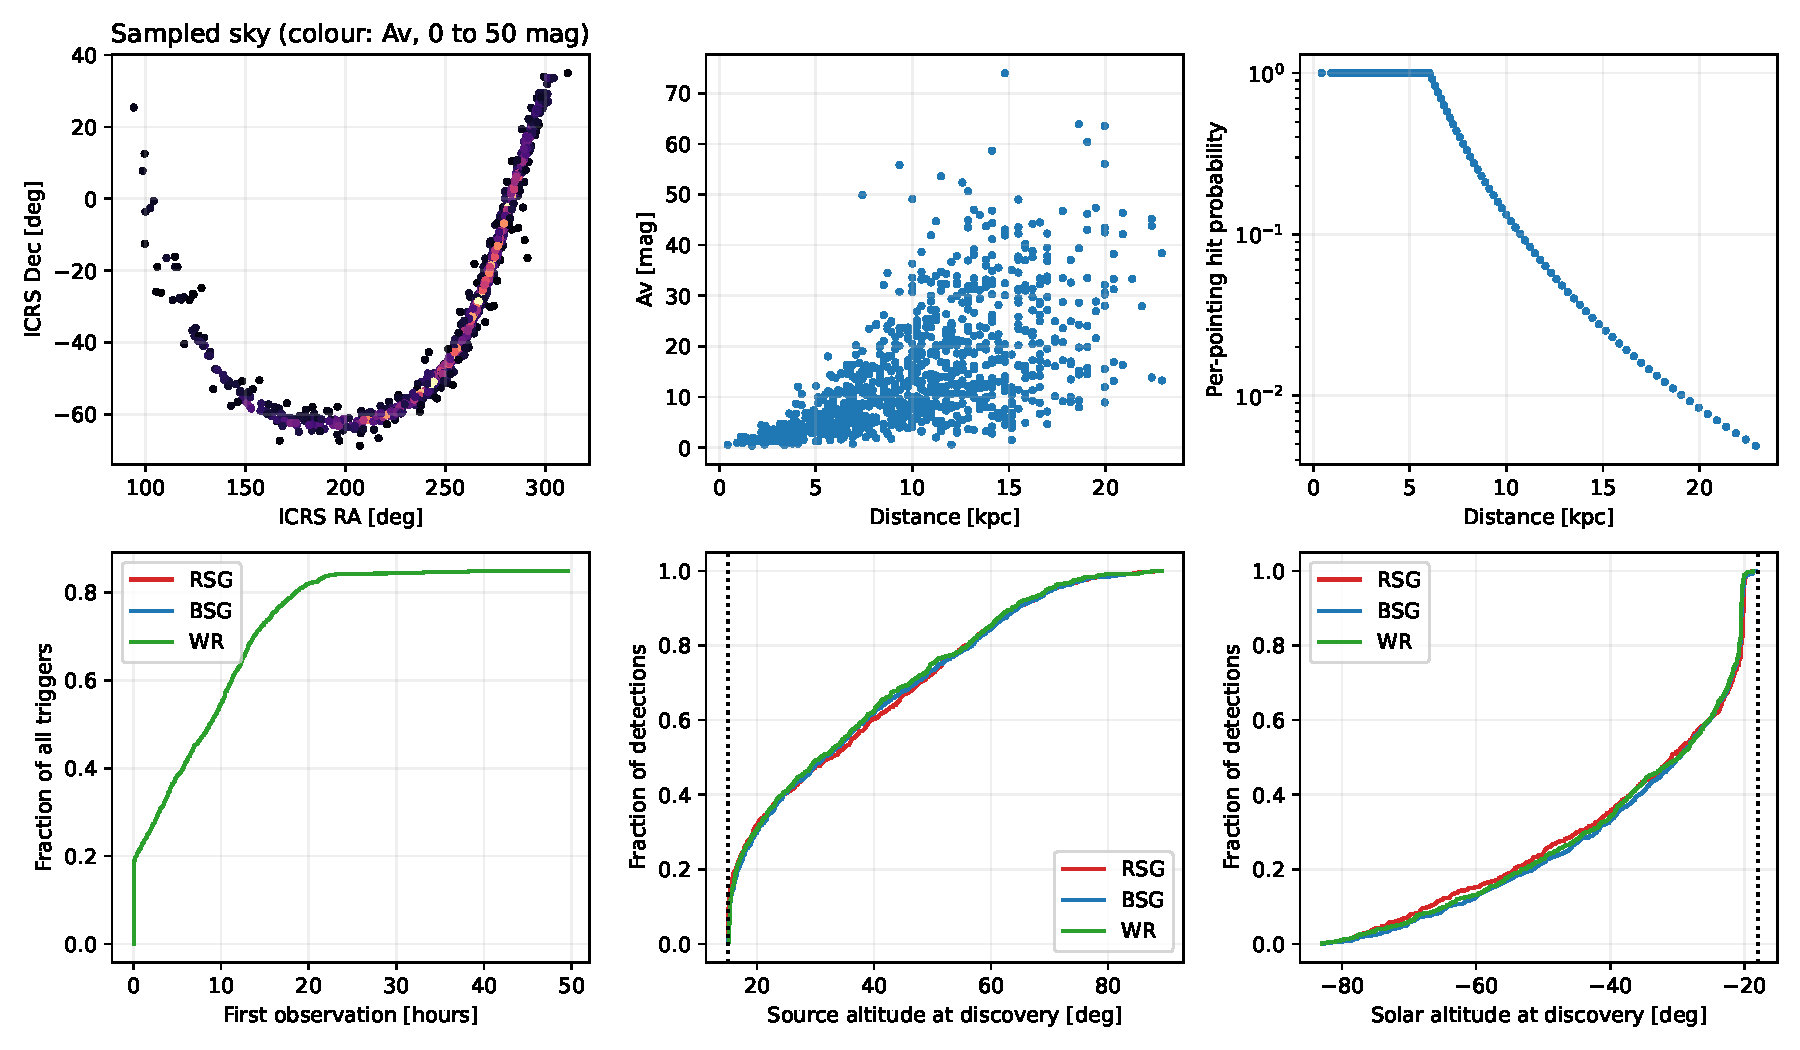
\includegraphics[width=\linewidth]{qa_population.pdf}
\caption{Population, extinction, localization and visibility diagnostics.
Shared inputs make first-observation distributions coincide across types.
All discovered events must satisfy the source and solar altitude cuts and
the Moon separation cut; the latter is checked separately against direct Astropy.}
\end{figure}
\begin{figure}[!htbp]\centering
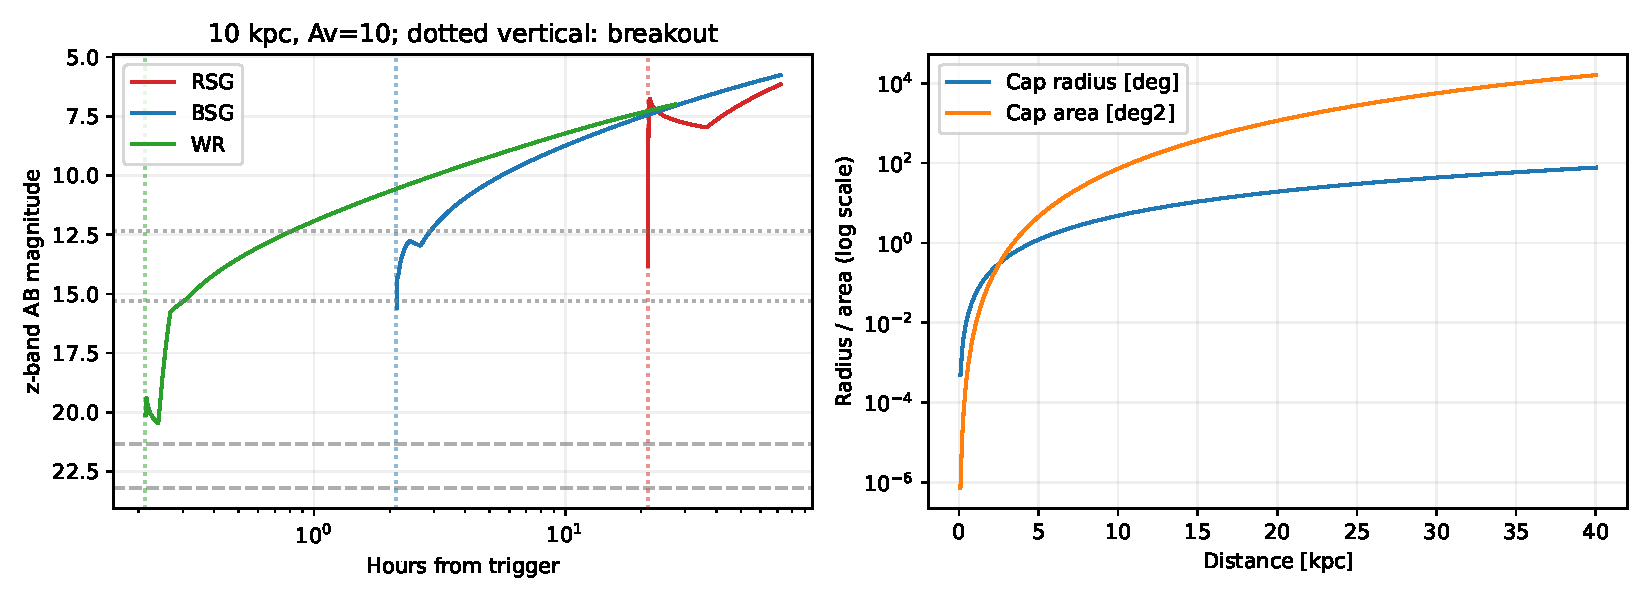
\includegraphics[width=\linewidth]{qa_models.pdf}
\caption{Reference light curves at 10 kpc and $A_V=10$, with detection (dashed)
and saturation (dotted horizontal) thresholds and breakout delays (vertical).
The right panel verifies localization scaling and the spherical-cap area.}
\end{figure}
\begin{figure}[!htbp]\centering
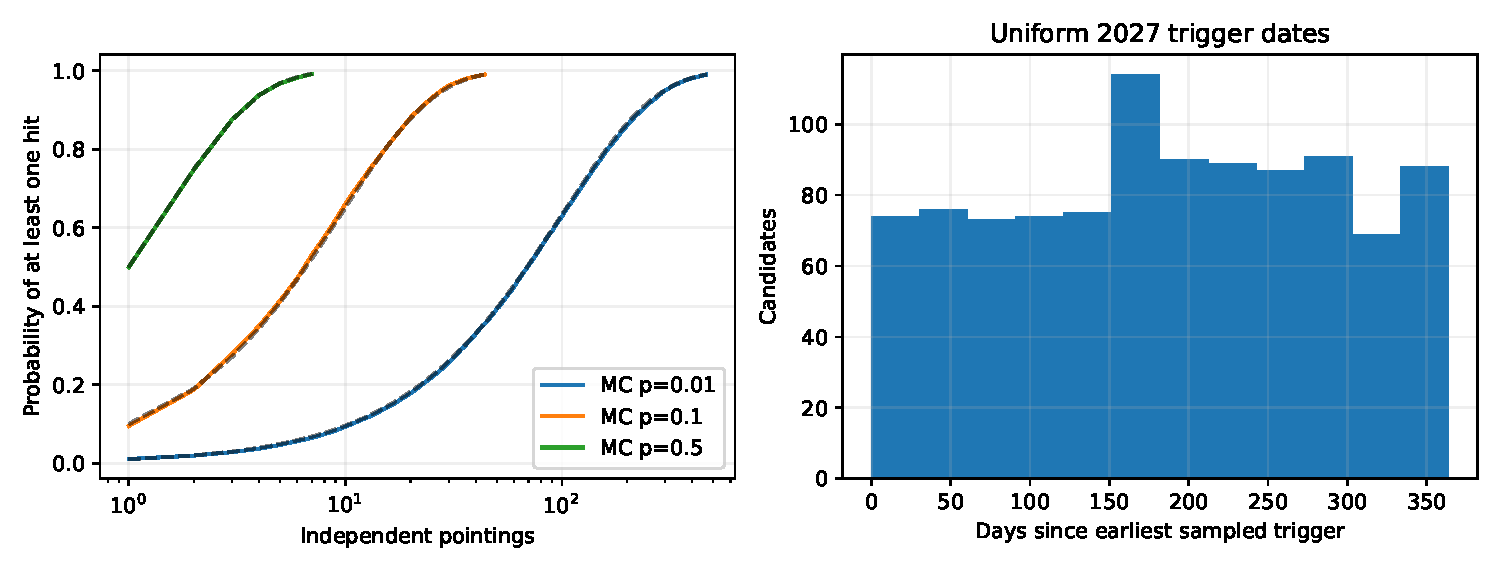
\includegraphics[width=\linewidth]{qa_sampling.pdf}
\caption{Independent search Monte Carlo against the geometric-distribution
prediction $1-(1-p)^N$ (dashed), and uniform trigger-date sampling.}
\end{figure}

Numerical tests cover cap geometry including full-sky capping, cadence and
setup, sensitivity and saturation scaling, direct SNR recovery, detection and
miss categories, tracking after discovery, mixed short/long saturation,
rapid rises between exposures, usable detections preceding later saturation,
invalid exposures preventing a fully saturated stop, flux integration and model validity,
Bernoulli hit statistics, distance conversion, reproducible catalogue sampling,
configuration validation, Moon-window clipping and disabling, lunar angle
wrapping, separation of nighttime and lunar failures, and astrometry against
direct Astropy AltAz positions
(0.02 degree absolute tolerance). Existing light-curve regression tests are run
alongside these integration tests. Full-run checks verify outcome accounting,
paired candidates, temporal limits and discovery geometry, including lunar
separation. Saved event diagnostics include the number of night/altitude
windows, complete pointings before and after the Moon veto, and the
source--Moon separation at discovery. The exposure audit retains individual
saturation flags, even when the event has usable photometry. The
\texttt{saturation\_s} field is the end of the first fully saturated pointing;
\texttt{immediate\_saturation} means that this is also the discovery pointing.
Neither field overrides the event's usable-photometry classification.

\clearpage
\section{Configurable parameters}
All simulation parameters are recorded below from the actual run configuration.
Six-entry instrument tuples use filter order $u,g,r,i,z,y$. Exposure tuples are
ordered, so the number of entries also configures the number of exposures.
CLI paths select the catalogue and output directory; their values and the
catalogue SHA256 are recorded in run metadata. Implementation choices described
above (e.g. uniform row sampling and independent search) are fixed model policies.
{\footnotesize\raggedright\input{\runpath/parameters.tex}}

\section{Reproduction and saved data}
Reproduction commands are in \texttt{GalSNRubin/README.md}.
\texttt{outputs/baseline\_moon/} stores all 3,000 outcomes
and supporting products. Audits cover the first three candidates per type.
Times ending in \texttt{\_s} are seconds from trigger; \texttt{trigger\_unix} is
UTC Unix time. \texttt{outputs/baseline/} retains the historical no-Moon run
with the old saturation rule.
\end{document}
